\begin{figure}
    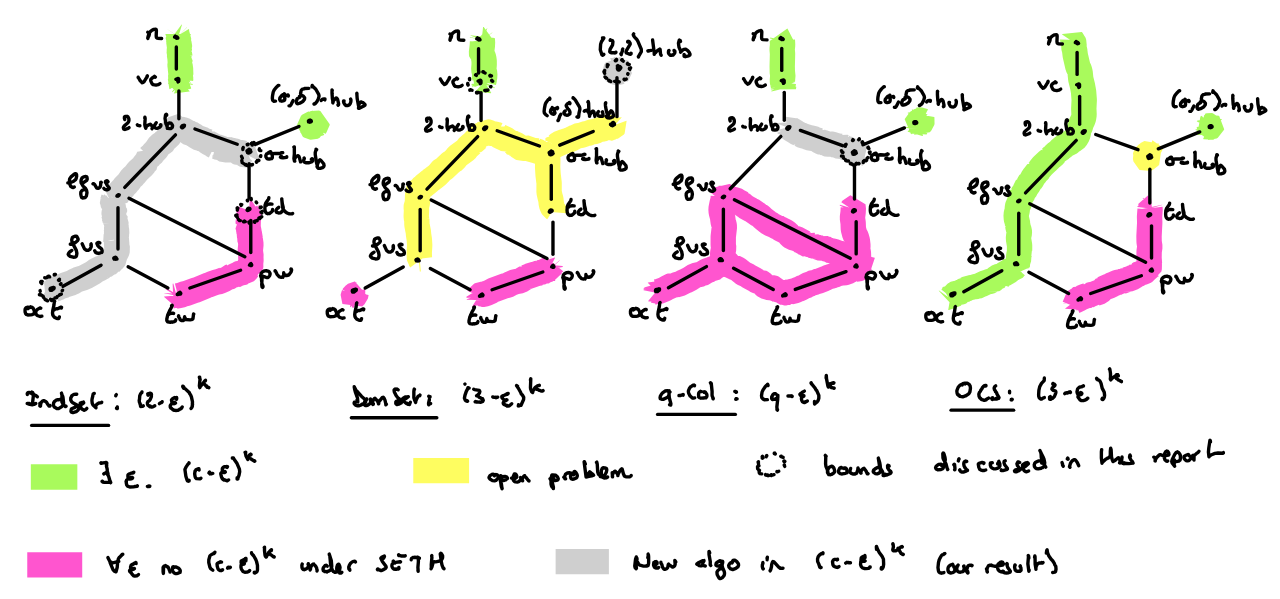
\includegraphics[width=\textwidth]{figures/state-of-the-art.png}
    \caption{Bounds for several \NP-hard problems. For each \NP-hard problem, we consider a constant $c$ and investigate whether there is an algorithm running in time $\O^\star((c-\varepsilon)^k)$ for some parameter $k$ and some $\varepsilon > 0$.}
    \label{fig:state-of-the-art}
\end{figure}